\section{A3Log System}
\label{sec:system}

In this section, we propose a Datalog System A3Log to support accumulate asynchronous aggregation, which is built by modifying Socialite \cite{Lam:2013:SDE:2510649.2511289,Seo:2013:DSD:2556549.2556572}. Datalog is an excellent candidate language for expressing computation logic because of its high-level \emph{declarative} semantics and support for recursion. In particular, Datalog program only defines how the output depends on the inputs but not how the outputs are produced. It operates on a relation at a time, exposing plenty of opportunities for parallelization and asynchronization by virtue of the size of the data sets, so that we have the flexibility to design specific runtime engines to support accumulate recursive program. \emph{automatic} parallelization and \emph{automatic} asynchronization. In addition, the program size of Datalog is much smaller than that of the imperative languages such as Java, C++. For these reasons, we choose Datalog as the high-level language.

\begin{figure}[!t]
    \centering
  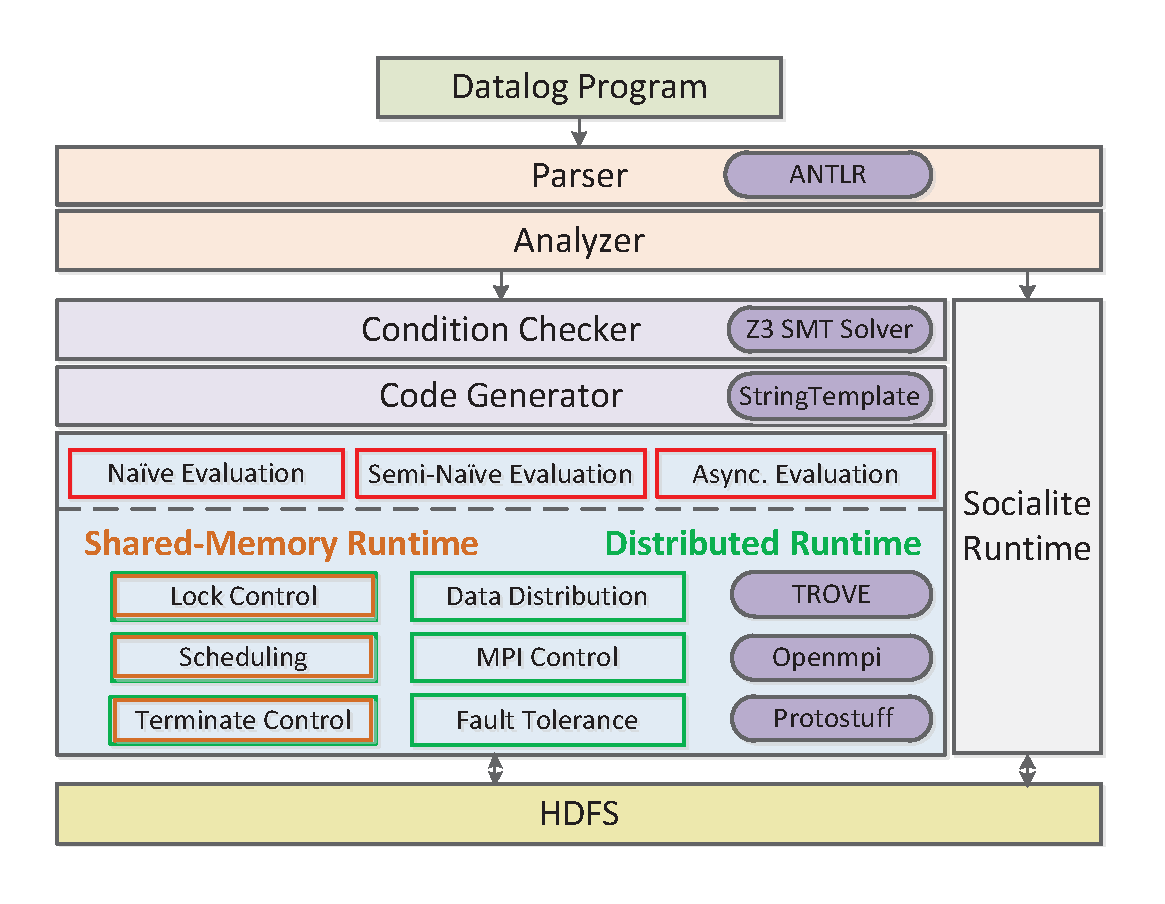
\includegraphics[width=3.2in]{fig/overview2}
  \vspace{-0.1in}
  \caption{A3Log overview NEED TO MODIFY}
  \label{fig:overview}
  \vspace{-0.2in}
\end{figure}

A3Log is implemented using Java and contains several components as shown in Fig. \ref{fig:overview}. The \textbf{Parser} parses user's Datalog program into an abstract syntax tree (AST) by using ANTLR \cite{antlr}. The \textbf{Analyzer} traverses the AST to performs syntactic and semantic analysis, identifies the recursive rule, and analyzes the aggregate operation $g$ and non-aggregate operation $f$. If the program is a recursive program, it will be further processed by our system, otherwise it will be executed by the Socialite runtime engine \cite{Lam:2013:SDE:2510649.2511289,Seo:2013:DSD:2556549.2556572}. Given the $f$ and $g$ operations retrieved by the Analyzer, the \textbf{Condition Checker} relies on Z3 SMT Solver \cite{DeMoura:2008:ZES:1792734.1792766,z3} to verify the conditions and automatically chooses the appropriate evaluation technique. The \textbf{Code Generator} provides a series of code templates for generating the share-memory runtime code and distributed runtime code, where we use StringTemplate \cite{stringtemplate} to generate source code. Then, the recursive program will be executed by our execution engine (Sec. \ref{sec:system:runtime}). A3Log provides both \textbf{Shared-Memory Runtime Engine} and \textbf{Distributed Runtime Engine}. The shared-memory runtime and distributed runtime share several functionalities, including lock control, scheduling, termination check. The distributed runtime additionally supports data distribution, MPI control, and fault tolerance. We use TROVE \cite{trove} for high performance container operations which are frequently used due to our key table structure, use openmpi \cite{mpich} for  communication, and use ProtoStuff \cite{kryo} for efficient serialization and deserialization. As implemented in Socialite, A3Log also relies on HDFS to store data and to checkpoint intermediate computation state.

\subsection{Datalog and Extension}
\label{sec:system:datalog}

A Datalog program is a set of rules. A \emph{rule} \texttt{r} has the form $h\leftarrow b_1,\ldots,b_n$, where $h$ is the \emph{head} and $b_1,\ldots,b_n$ is the \emph{body}. The comma separating literals in a body is a logical conjunction (AND). $h$ and $b_i$ can be with the form $p_i(t_1,\ldots,t_j)$ where $p_i$ is a \emph{predicate} and $t_1,\ldots,t_j$ are terms which can be \emph{constants}, \emph{variables} or \emph{functions}. For example, the Datalog program for SSSP computation can be written as follows.
%The data associated with abstract predicate is referred to as \emph{fact}.

\begin{verbatim}
Program 1. Single Source Shortest Path
\end{verbatim}
\vspace{-0.1in}
\small
\begin{lstlisting}
r1. sssp(X,$d$)$\leftarrow$ X=1,$d=0$.
r2. sssp(Y,min[$d$])$\leftarrow$ sssp(X,$d1$),edge(X,Y,$d2$),
		     $d=d1+d2$,sssp(Y,$d$).
\end{lstlisting}
\normalsize

In Program 1, rule \texttt{r1} initializes the predicate \texttt{sssp} by specifying the source node $X=1$ and the shortest distance from source as $d=0$. \texttt{r2} is a recursive rule since it has the \texttt{sssp} predicate in both its head and body. \texttt{r2} will recursively produce \texttt{sssp} fact by joining the old \texttt{sssp} and \texttt{edge}. If there is a path from source to $X$ of length $d_1$ and an edge from $X$ to $Y$ of length $d_2$, there is a path from source to $Y$ with length $d=d_1+d_2$. If there is already a path to $Y$ found before, it should be also considered. Hence, the shortest distance from source to $Y$ is updated by the minimum of these possible distances, i.e., min$[d]$. The recursion will terminate as soon as no shortest distance is updated.

Originally, the Datalog program terminates when no new fact can be found. However, some programs will never stop since it continuously produces ``tiny'' facts. For example, the PageRank computation will continuously update the PageRank scores even though the changes are less and less. In order to help users express more termination conditions, we allow users to specify the termination conditions using aggregations.


\begin{verbatim}
Program 2 PageRank
\end{verbatim}
\vspace{-0.1in}
\small
\begin{lstlisting}
r1. degree(X,count[Y])$\leftarrow$ edge(X,Y).
r2. rank(X,$r$) $\leftarrow$ node(X),$r=1$.
r3. rank(Y,sum[$r$]+0.15) $\leftarrow$ rank(X,$r1$),edge(X,Y),
			degree(X,$d$),$r=0.85\cdot r1/d$,
			[sum$[\Delta r]\leq 0.001$].
\end{lstlisting}
\normalsize

In Program 2, we show the Datalog program for PageRank. \texttt{r1} computes the node degrees based on the edge data. \texttt{r2} initializes the predicate \texttt{rank} by specifying all the nodes' ranking scores as a constant 1. \texttt{r3} is a recursive rule that updates the predicate \texttt{rank}. We allow users to specify the terminate conditions in $[\ldots]$ by using different aggregate operations. In this program, the PageRank computation will terminate when the sum of ranking score differences of two continuous recursion results is less than or equal to 0.001.

Besides SSSP and PageRank, we list 11 more example Datalog programs that can be executed asynchronously in the Appendix Sec. \ref{sec:app:example}. These examples cover a wide range of applications, including graph analytics (Program 3, 4, 5, 12), data mining (Program 6, 7, 9, 10), machine learning (Program 8, 11), and HPC (Program 13).

\subsection{Condition Checker}
\label{sec:system:condition}

\begin{figure}[!t]
    \centering
  \includegraphics[width=2.8in]{fig/flow}
  \vspace{-0.1in}
  \caption{Condition checking flow chart}
  \label{fig:flow}
  \vspace{-0.2in}
\end{figure}

A3Log is able to automatically verify the conditions for asynchronous aggregation and accordingly selects the appropriate optimization technique according to the satisfiable conditions. The $g$ operation is identified as the update operation in the recursive rule's head predicate, e.g., min[$d$] in SSSP and sum[$r$]+0.15 in PageRank where [$d$] and [$r$] are the inputs, respectively. The $f$ operation is identified as the computation in the recursive rule's certain body predicate that updates the input variables of $g$ operation, e.g., $d=d1+d2$ in SSSP and $r=0.85\cdot r1/d$ in PageRank. The input variable of $f$ operation is the variable that appears in the recursive predicate, e.g., $d1$ in \texttt{sssp(X,$d1$)} and $r1$ in \texttt{rank(X,$r1$)}.

There are two techniques for executing recursive Datalog programs. The first is \emph{\textbf{Naive Evaluation}}. For instance, in Program 1, the recursive rule \texttt{r2} will be repeatedly evaluated. The \texttt{edge} facts keep being joined with the \texttt{sssp} facts discovered so far in each iteration, until no new fact is produced. This approach will inefficiently re-produce known facts in every iteration. To address this inefficiency issue, the \emph{\textbf{Semi-Naive Evaluation}} for recursive programs with aggregation was proposed \cite{Lam:2013:SDE:2510649.2511289,Wang:2015:AFR:2824032.2824052}, which is efficient and produces no duplicates. However, the semi-naive evaluation requires the program to be set-containment monotonic in order to guarantee the correctness. This is the same as the monotonizability condition that we have defined in Theorem \ref{th:monotone}. Therefore, as long as the program satisfies monotonizability condition or can be converted to be monotonic according to Theorem \ref{th:convert}, it can be executed with semi-naive evaluation. Furthermore, we propose \emph{\textbf{asynchronous evaluation}} as a yet another optimization technique, which allows asynchronous aggregation. We provide the sufficient conditions for asynchronous aggregation in Theorem \ref{th:async}. The prerequisite for asynchronous aggregation is the monotonic condition. Asynchronous evaluation is possible only when the recursive program is monotonic and satisfies order independent condition.

Condition Checker first translates the $f$ and $g$ operations into Z3 \cite{DeMoura:2008:ZES:1792734.1792766} satisfiability formulas (see Sec. \ref{sec:async:autoasync}). By applying $f$ and $g$ to the built-in condition checking templates, the Z3 SMT olver will answer satisfiable, unsatisfiable, or unknown. Following the condition checking flow as shown in Fig. \ref{fig:flow}, our system can automatically select the appropriate evaluation technique.

\subsection{Key Data Structure: AsyncTable}
\label{sec:system:data}

Before launching the recursive computation, the key table structure, AsyncTable, should be first prepared. AsyncTable maintains the computation states, which are initialized based on user's Datalog program and keeps being updated during the whole recursive computation process.

\begin{figure}[!t]
    \centering
  \includegraphics[width=3.2in]{fig/asynctable}
  \vspace{-0.1in}
  \caption{AsyncTable update}
  \label{fig:asynctable}
  \vspace{-0.2in}
\end{figure}


\noindent\textbf{AsyncTable Design}
As shown in Fig. \ref{fig:asynctable}, the AsyncTable contains several columns. The main key column and accumulation column store the result key-value pairs. The main key entries index the table. The accumulation column entry monotonically aggregates the intermediate results and maintains $g(\Delta x^0,\Delta x^1,\ldots)$. The accumulative property of $g$ operation makes it possible to use a single column to maintain all the intermediate results,i.e. The intermediate column entry stores the temporary aggregation results $g(\Delta X^k)$ which will be used to generate future intermediate results by applying $f$ operation. The auxiliary columns store the data which might be used by the $f$ or $g$ operation, e.g., outgoing neighbors set in SSSP and the node degree value in PageRank. The accumulation column entries and intermediate column entries are volatile, which maintain the computation states and keep being updated during the computation, while the other column entries are fixed after initialization. The AsyncTable is sharded for parallel processing. Each shard contains a number of rows and is assigned to a compute thread or placed on a distributed worker machine.

\noindent\textbf{AsyncTable Initialization}
The AsyncTable is initialized according to user's program. The recursive rule head contains the main key and accumulation column's information. For example in SSSP, the main key column entries are initialized with the node ids. The accumulation column is initialized with the identity element \textbf{0} w.r.t $g$, e.g., MAX in SSSP. The intermediate column is initialized in terms of the non-recursive rule \texttt{r1}, i.e., 0 for the source node and MAX for other nodes. The auxiliary data dependency column is identified as the rule body predicate that describes the relationship between main keys, e.g., \texttt{edge(X,Y,d2)}. The auxiliary variable column entries can be identified as the joined results between rule body predicates, e.g., the degree information \texttt{d} in PageRank.

A few additional facts should be noticed: 1) It is possible that two or more items are identified as the main key (see Program 4, 5, and 12 in Appendix Sec. \ref{sec:app:example}); 2) The AsyncTable size can be dynamic rather than fixed due to the continuously inserted new rows (see Program 4, 5, 7, and 9); 3) The recursive program can be composed of more than one interdependent rules, which can be reduced to one rule (see Program 9 and 10).

\subsection{Execution Runtime Engine}
\label{sec:system:runtime}

\begin{figure}[!t]
    \centering
  \includegraphics[width=2.9in]{fig/runtime}
  \vspace{-0.1in}
  \caption{Execution Runtime Engine}
  \label{fig:runtime}
  \vspace{-0.1in}
\end{figure}

\noindent\textbf{Overall Architecure}
A3Log provides both shared-memo-ry runtime engine and distributed runtime engine. Fig. \ref{fig:runtime} shows the overall structure. The shared-memory runtime has a simple design. A number of compute threads are created to update the AsyncTable in parallel, and a termination check thread is running separately to check the stop condition. The distributed runtime contains a number of workers and a master worker. Each worker creates a number of compute threads to update the local AsyncTable shard. A communicate thread tackles the remote update. We adopt a send buffer design to control the overhead of frequent communications. The master worker creates a termination check thread to globally check stop condition periodically.


\noindent\textbf{Concurrency Control}
The accumulation column entries and intermediate column entries keep being updated during computation. Specifically, an intermediate column entry is read to update the same row's accumulation column entry (by operation 1 in Fig. \ref{fig:asynctable}) and to update other rows' intermediate column entries (by operation 2 in Fig. \ref{fig:asynctable}), and is reset as \textbf{0} (by operation 3 in Fig. \ref{fig:asynctable}). The reset operation is essential to make result correct, without which the same intermediate result would be redundantly accumulated. These three operations have to be \emph{atomic} according to the definition of accumulated recursive program (Definition \ref{eq:accumasync}). However, an intermediate column entry can be read and written concurrently by multiple threads or multiple workers, which leads to potential consistency problem. In our shared-memory runtime, we use \emph{optimistic} lock to avoid read-write conflicts. In distributed runtime, the consistency problem will happen in the send buffer, which maintains the remote updates. The optimistic lock does not work well since the communicate thread is required to serialize the whole buffer for efficiency and the lock granularity becomes too coarse to result in too many aborts. We employ MVCC (multi-version concurrency control) to address this problem. Specifically, we adopt a double-version design of the send buffer, which serves the compute threads and communicate thread alternatively.


\noindent\textbf{Scheduling}
When executed in synchronous module,There is no necessary or chance to schedule the computing.But in asynchronous module.The clever scheduling of aggregate operations has the potential of accelerating the convergence of recursive computations.The scheduling should be performed by evaluating the intermediate aggregation result (intermediate column entries in AsyncTable). The top intermediate column entries (in the partial order defined by $g$) should be scheduled. Since the intermediate column entries keep being pdated, the top entries should be evaluated frequently. For the sake of reducing scheuduling cost, we utilize the sampling technique \cite{Zhang:2011:PDF:2038916.2038929} to approximately obtain the top $N\%$ entries. The scheduling is even more costly in distributed environment. Rather than global scheduling, local scheduling in each worker is preferred.
%The portion ($N\%$) of entries to be scheduled balances the tradeoff between the optimal scheduling benefit and the sorting cost. We will empirically study the effect of $N\%$ in Sec. \ref{sec:expr:schedle}.

\noindent\textbf{Termination Check}
The termination condition might rely on aggregation of either the accumulation column entries or the intermediate column entries. The aggregation is evaluated by the termination check thread without disturbing the compute threads. While in distributed runtime, each worker will report their local aggregation results to the master, where the global termination check thread determines whether to stop by evaluating the global aggregation result. Note that, there is no iteration's conception in asynchronous aggregation, so we have to check the termination condition every other period of time rather than every other iteration.

\noindent\textbf{Fault Tolerance}
For large scale operations that involve many machines for a substantial amount of time, it is also important to provide fault tolerance support. A3Log relies on Socialite's fault tolerance scheme \cite{Seo:2013:DSD:2556549.2556572}. The intermediate computation states are checkpointed occasionally on HDFS and restorable as needed. If one or more workers fail, the intermediate states are restored from the latest checkpoint and the evaluation is resumed from that point.

